% !TeX root = Par_paket.tex
%!TEX program = lualatex

\documentclass[12pt]{exam} %addpoints, togs bort för att testa andra poäng
\usepackage[swedish]{babel}
%\usepackage[utf8]{inputenc}
\usepackage[T1]{fontenc}
\usepackage{mathtools}
\usepackage{amssymb}
\usepackage{amsthm}
\usepackage{kmath}
\usepackage{kerkis}
\usepackage{systeme}
\usepackage{graphicx}
\usepackage[parfill]{parskip}
\usepackage[a4paper,left=1cm, right=1cm,top=1.5cm, bottom=2cm]{geometry}
\usepackage{siunitx}
\usepackage{enumitem}
\usepackage{multicol}
\usepackage[sharp]{easylist}
\usepackage{pgfplots}
\pgfplotsset{compat=1.8}
\usepgfplotslibrary{statistics}
\usepackage{tkz-euclide}
\usetikzlibrary{colorbrewer}
\usetikzlibrary{arrows}
\usepackage{caption}
\usepackage{subcaption}
\usepackage{float}
\usepackage{xcolor}
\usepackage{setspace}
\usepackage{datatool}
%\DTLloaddb{koder}{test.txt}
\usepackage[sc]{titlesec}
\usepackage{tabularray}
\usepackage[strict]{changepage}
\usepackage{wrapfig}
\usepackage{emoji}
\setemojifont{TwemojiMozilla}
\usepackage{caption}


\usepackage[most]{tcolorbox} 
\definecolor{block-gray}{gray}{0.95}


\newtcolorbox{zitat}[2][]{%
    colback=block-gray,
    grow to right by=-10mm,
    grow to left by=-10mm, 
    boxrule=0pt,
    boxsep=0pt,
    breakable,
    enhanced jigsaw,
    borderline west={4pt}{0pt}{gray},
    title={#2\par},
    colbacktitle={block-gray},
    coltitle={black},
    fonttitle={\large\bfseries},
    attach title to upper={},
    #1,
    text width=4.5cm,
}


\renewcommand\qedsymbol{$\blacksquare$} % namn till olika text miljöer
\theoremstyle{plain}% default
\newtheorem{thm}{Sats}
\newtheorem{lem}[thm]{Lemma}
\newtheorem{prop}[thm]{Proposition}
\newtheorem*{cor}{Korollarium}


\theoremstyle{definition}
\newtheorem{defn}{Definition}
\newtheorem{exmp}{Exempel}
\newtheorem{upg}[exmp]{Uppgift}

\theoremstyle{remark}
\newtheorem*{rem}{Tips}
\newtheorem*{note}{Anmärkning}

\everymath{\displaystyle}


\colorgrids % gör att svarsrutnäten är ljusgrå
\colorfillwithdottedlines
\setlength{\gridlinewidth}{0.7pt}
\definecolor{GridColor}{gray}{0.9}
%\pointsinrightmargin 
\setlength{\rightpointsmargin}{2cm}
%\pointformat{\fbox{\phantom{\themarginpoints }/\themarginpoints}}
\marginpointname{}

% Svenska namn till poänglista
%\pointpoints{Poäng}{Poäng}
%\bonuspointpoints{Bonuspoäng}{Bonuspoäng}
\pointpoints{}{}
\bonuspointpoints{}{}
\totalformat{Uppgift \thequestion: \totalpoints{} poäng}
\hqword{Uppgift:}
\hpgword{Sida:}
\hpword{Poäng:}
\hsword{Resultat:}
\htword{Total}

%För att skriva ut fråge namn och inga siffror
\qformat{\sc\thequestiontitle\dotfill\thepoints 
\vrule depth 1em width 0pt
} 

\newcommand{\mild}{\emoji{hot-pepper}}
\newcommand{\medel}{\emoji{hot-pepper}\emoji{hot-pepper}}
\newcommand{\het}{\emoji{hot-pepper}\emoji{hot-pepper}\emoji{hot-pepper}}

\firstpageheader{\bfseries Inlämning utkast:\draft , Slutlig:\final}{}{\large\bfseries Namn:\enspace\makebox[2in]{\hrulefill}}
\runningheader{}{}{\oddeven{\large\bfseries Namn:\enspace\makebox[2in]{\hrulefill}}{}}% skriver bara ut namn på varanan sida. Dvs en gång per papper vid dubbelsidig utrskrift.

\firstpagefooter{\class}{\thepage\ (\numpages)}{}
\runningfooter{\class}{\thepage\ (\numpages)}{}


\newcommand{\ovning}{
\usepackage{draftwatermark}
\SetWatermarkColor{red!10}
\SetWatermarkScale{1}
\SetWatermarkText{Övning}     %Watermark text
%\usepackage{pgfmorepages}
%\pgfmorepagesloadextralayouts
%\pgfpagesuselayout{repeated 2-up}[a4paper,landscape]
}


% For an exam, single spacing is most appropriate
\singlespacing
% \onehalfspacing
% \doublespacing


%%%% Inställningar för provet %%%%

% Kommentera bort om det inte ska stå övning på provet
%\ovning 

\newcommand{\class}{Ma2c}
\newcommand{\term}{HT 24}
\newcommand{\nummer}{1}
\newcommand{\draft}{17/5}
\newcommand{\final}{19/5}
%\newcommand{\timelimit}{15 minuter} 
%\newcommand{\hjalp}{Chromebook med geogebra / Räknare, Formelsamling} % I minuter
\pgfmathdeclarefunction{gauss}{2}{%
  \pgfmathparse{1/(#2*sqrt(2*pi))*exp(-((x-#1)^2)/(2*#2^2))}%
}
\sisetup{locale = DE}

\begin{document}
\begin{center}
{\Large \textsc{PAR Problem nr.}\nummer}\\[0.3cm]
\end{center}

\fbox{\fbox{\parbox{\textwidth}{{
\noindent \centering PAR Processen\\
Skriv ett utkast \hspace{0.3cm} Reflektera \hspace{1.1cm} Feedback \hspace{1.3cm} Förbättra \hspace{1.2cm} Lämna in \phantom{te}\\
\includegraphics*[width=15cm]{img/par_prosess.png}\\}
\phantom{testtesttset}(Hemma) \hspace{1.4cm} (Hemma) \hspace{0.5cm} (Fredags lektionen) \hspace{0.3cm} (Hemma) \hspace{0.5cm} (Tisdags lektionen) }}}
\smallskip \vspace{0.5cm}

    


% -------------------------------------------------------------

%Here, the questions begin
\begin{questions}
\setlength\itemsep{2\baselineskip}
\titledquestion{Kvadrater i kvadrat}[\mild]

Lös ekvationen $$(x^2-7x+11)^{(x^2-11x+30)}=1$$.

\begin{rem}
    Om du vet att två tal uppfyller $a^b=1$ vad kan du säga om talen $a$ och $b$.
\end{rem}

\titledquestion{100 Meters loppet}
Alice, Bob och Charlie ska tävla på 100 m löpning. Alice är snabbare än Bob och Charlie. Bob har inte tävlat på 100m tidigare så han får ett försprång för att de alla ska ha en chans att vinna.
På träning brukar Alice springa 100 meter på 10-11 sekunder. Bob har de få gånger han testat tagit längre tid på sig, 12-13 sekunder. 

\begin{figure}[H]
    \centering
    \includegraphics[width=0.8\linewidth]{img/löpbana.png}
\end{figure}

\begin{parts}
  
  \part Baserat på deras tidigare tider, hur lång tid tror du Alice, respektive Bob tar att springa 100 m?
  \part Hur många meters försprång borde Bob få för att det ska bli ''rättvist'', dvs både Alice och Bob ska ha en chans att vinna?
  \part Vem kommer på första, andra och sista plats? Förklara tydligt vilka antaganden du gör?
  \part Rita in de tre löparnas position som funktion av tiden i ett koordinatsystem. Se till att dina grafter stämmer med de antaganden du gjort.
\end{parts} %Ändra till den uppgift som ska byggas

\titledquestion{K-värde eller värde av k?}

Ekvationen $2x + ky = -k$ beskriver en rät linje. För varje deluppgift bestäm om de finns värden på konstanten $k$ så att linjen uppfyller kravet samt vilka värden detta är.
\begin{parts}
  \part Linjen har riktningskoefficienten (lutningen) 3.
  \part Linjen går genom punkten $(0,-1)$
  \part Linjen är horisontell.
  \part Linjen är vertikal.
  \part Linjen passerar inom 1 l.e. av origo.
\end{parts} 

\titledquestion{Tre punkter}

De tre punkterna $A = (-3, 1)$, $B = (1, 3)$ och $C = (-1, 5)$ utgör hörn i en triangel.
\begin{parts}
    \part Bestäm ekvationen till linjen som utgör förlängningen av sidan $AB$.
    \part Hitta ekvationen till linjen som utgör förlängningen av triangelns höjd genom hörnet $C$.\\
    (Höjden är vinkelrät mot basen, i detta fall sidan $AB$)
    \part Bestäm skärningspunkten mellan sidan $AB$ och höjden du fick fram i (b).
    \part[\mild] Bestäm triangelns area.
\end{parts}

\input{uppgifter/Lösa ekvationssystem.tex}

\titledquestion{Mix av vektorer}

Med hjälp av olika kombinationer av två givna vektorer kan man skapa alla andra vektorer, förutsatt att de två givna vektorerna inte är parallella.

\begin{figure}[H]
    \centering
    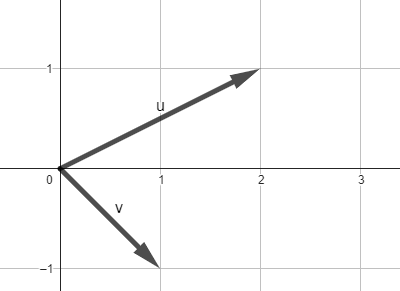
\includegraphics[width=0.5\linewidth]{img/vektorer.png}
    \caption{De två givna vektorerna.}
\end{figure}

\begin{parts}
    \part Skriv upp $\vec{u}$ och $\vec{v}$ på koordinatform.
    \part Uttryck vektorn $\vec{w}=(0,3)$ med hjälp av $\vec{u}$ och $\vec{v}$. Lös uppgiften både grafiskt och algebraiskt. 
    \part Uttryck vektorn $\vec{t}=(11,10)$ med hjälp av $\vec{u}$ och $\vec{v}$. 
    \begin{rem}
        Vi har nyss lärt oss ekvationssystem...
    \end{rem}
\end{parts} 

\titledquestion{Sangaku}

Sangakus är en typ av japanska (ofta geometriska) matematikproblem som under Edo perioden lämnades vid tempel som en form av offergåva.

En av de kändaste har att göra med tre cirklar som alla tangerar varandra och en linje.
\begin{figure}[H]
    \centering
    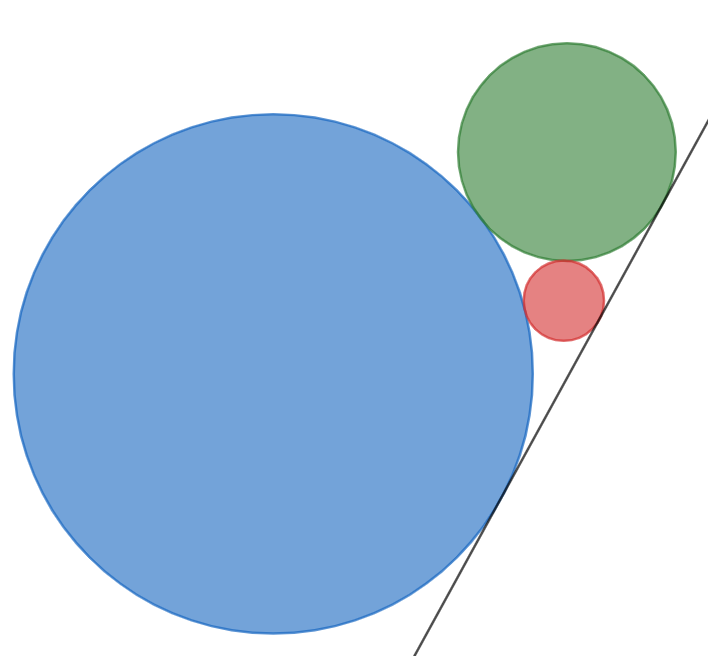
\includegraphics[width=0.5\linewidth]{img/tre cirklar.png}
    \caption{Tre cirklar som alla tangerar en linje.}
\end{figure}


Radien av den gröna cirkeln är 9 cm, och radien av den blå är 36 cm.

Vilken radie har den röda cirkeln?

\begin{rem}
    Kan du räkna ut ''höjdskillnaden'' mellan centrum för den blå och den gröna cirkeln?\\
    Kan du räkna ut hur långt det är mellan de punkter där den blå och den gröna cirkeln tangerar linjen?
\end{rem} 

\titledquestion{Kvadrater i kvadrat}[\mild]

Lös ekvationen $$(x^2-7x+11)^{(x^2-11x+30)}=1$$.

\begin{rem}
    Om du vet att två tal uppfyller $a^b=1$ vad kan du säga om talen $a$ och $b$.
\end{rem}

\titledquestion{Vertex}

\begin{boxdef*}{Vertex}
  Vertex är den eller de punkt(er) där en kurva vänder ''håll''. Kurvan av en andragradsfunktion har en vändpunkt. Kurvor av högre grader kan ha flera.
  Ordet vertex är latin med betydelsen ''topp-punkt, vändpunkt''.
\end{boxdef*}

Denna vecka ska vi undersöka hur koefficienten för $x$ påverkar grafen till parabeln $y=3x^2 +bx-2$.

\begin{parts}
  \part Vi börjar med att betrakta positiva värden på $b$. Plotta $y=3x^2 +x-2$, $y=3x^2 +2x-2$ och $y=3x^2 +6x-2$ i samma koordinatsystem. Beskriv hur värdet på $b$ påverkar
  vertex för parabeln. Testa gärna fler värden på $b$ om du ännu inte känner dig säker på dina observationer.

  \part Plotta nu $y=3x^2 +bx-2$ för $b = -1, -2 \text{ och } -3$. När koefficienten är negativ, hur påverkar dess värde kurvans vertex?

  \part Baserat på dina svar i (a) och (b) beskriv hur värdet på $b$ påverkar positionen för vertex. Ditt svar ska gälla för alla värden på $b$, positiva, negativa och noll.

  \part Alla de plottar du gjort skär y-axeln i samma punkt. Ge en enkel förklaring varför detta sker.

\end{parts}

\titledquestion{Vertexform}[\medel]

Alla andragradsfunktioner $y=ax^2 +bx+c$ kan via kvadratkomplettering skrivas på vertexform, $y=A(x-B)^2+C$ där $A,B \text{ och } C$ är konstanter. 

Skriv om funktionen i första uppgiften på vertexform och jämför med de slutsatser om positionen av vertex du drog i första uppgiften.
 

\titledquestion{Triangelns vinkelsumma}
Denna vecka ska vi öva på att föra geometriska resonemang. Uppgifterna kommer endast att kräva det som står under ''Vinklar'' på formelbladet. 

En linje ritas genom ett av hörnen på en triangel så att linjen är parallel med motstående sida. Se figur 1.

\begin{figure}[H]
    \centering
    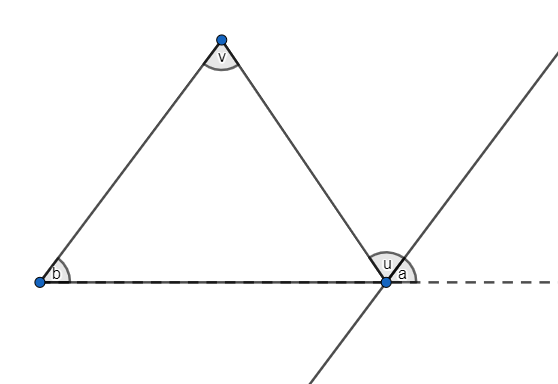
\includegraphics[width=0.5\linewidth]{img/prop32.png}
    \caption{}
\end{figure}

\begin{parts}
  \part Visa att vinklarna $a$ och $b$ är lika stora.
  \part Visa att vinklarna $v$ och $u$ är lika stora.
  \part Visa att triangelns vinkelsumma är \ang{180}.
  \part Visa att yttervinkeln i en triangel är lika med summan av de två motstående innervinklarna. 
\end{parts}


\titledquestion{Vinklar i ett parallellogram}
En parallellogram är en fyrhörning där motstående sidor är parallella.

\begin{parts}
  \part Visa att motstående vinklar i en parallellogram är lika stora.
  \part[\het] Visa att om motstående vinklar i en fyrhörning är lika stora så är fyrhörningen en parallellogram.
\end{parts} 

\titledquestion{Glasspaketet}
De hungriga ungdomarna Asta, Bea och Cesar ska dela på ett glasspaket. Diskussionen uppstår då hur
paketet ska delas rättvist. På kanten finns en markering som de förstår är mitten av paketet (E). Asta
drar då två sträckor utifrån den mittpunkten (AE) samt paketets hörn (BD) (de streckade sträckorna på bilden) och skär sedan av paketet i
skärningspunkten (F) och påstår att hon tagit exakt en tredjedel, den bit som utgörs av fyrhörningen ABHG.
Stämmer det?
\begin{figure}[H]
    \centering
    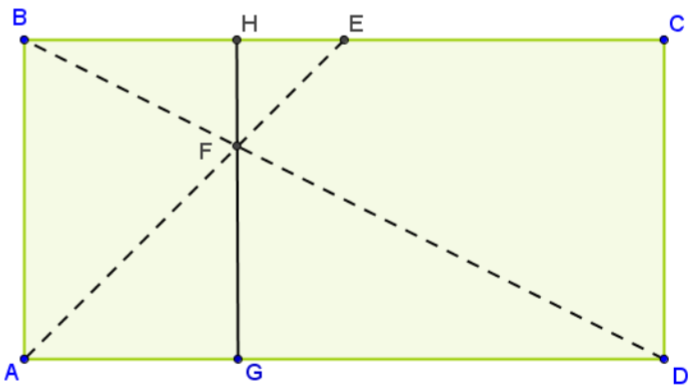
\includegraphics[width=0.5\linewidth]{img/Glasspaket.png}
    \caption{Ett glasspaket.}
\end{figure} 
%-------------------------------------------------------------------
%Här kommer svars områden och sånt
\newpage
\begin{center}
  Feedback av:\enspace\makebox[2in]{\hrulefill}\\
\end{center}

\smallskip
\noindent Styrkor \hfill Kommunikation \hfill Förslag \hrule

\begin{figure}[H]
    \centering
    \caption*{}
    
\includegraphics[width=1.5cm, page=3]{img/Bilder.pdf}
    \caption*{Lätt att följa alla steg.}
    \smallskip
    
\includegraphics[width=1.5cm, page=2]{img/Bilder.pdf}
    \caption*{Förklarar varför,\\ inte bara vad.}
    
\includegraphics[width=1.5cm, page=1]{img/Bilder.pdf}
    \caption*{Använder namn.}
    
\includegraphics[width=1.5cm, page=5]{img/Bilder.pdf}
    \caption*{Tydliga definitioner av variabler.}
    
\includegraphics[width=1.5cm, page=6]{img/Bilder.pdf}
    \caption*{Använder diagram.}
\end{figure}

\noindent Styrkor \hfill Korrekthet \hfill Förslag \hrule
\begin{figure}[H]
  \centering
  \caption*{}
  
\includegraphics[width=1.5cm, page=8]{img/Bilder.pdf}
  \caption*{Korrekta beräkningar}
  
\includegraphics[width=1.5cm, page=9]{img/Bilder.pdf}
  \caption*{Testat olika sätt.}
  
\includegraphics[width=1.5cm, page=10]{img/Bilder.pdf}
  \caption*{Rimligt svar.}

\end{figure}
\newpage
\section*{Utkast}
\fillwithgrid{\stretch{1}}
\newpage
\fillwithgrid{\stretch{1}}
\newpage
\section*{Slutinlämning}
\fillwithgrid{\stretch{1}}
\newpage
\fillwithgrid{\stretch{1}}


\end{questions}
\end{document}
